% !TeX program = xelatex
% !TeX options = -shell-escape
% !TEX encoding = UTF-8

% --------------------------------------------------------------
% This is all preamble stuff that you don't have to worry about.
% Head down to where it says "Start here"
% --------------------------------------------------------------

\documentclass[12pt]{article}
\usepackage[margin=2cm]{geometry} % 頁面邊距設置
\usepackage{amsmath,amssymb,amsthm} % 數學相關套件
\usepackage{graphicx} % 圖形插入
\usepackage{booktabs} % 表格線條
\usepackage[AutoFakeBold,AutoFakeSlant]{xeCJK} % 中文支援
\usepackage{fancyhdr} % 頁首頁尾設置
\usepackage{xcolor,changepage,mdframed} % 顏色與框線相關
\usepackage{titlesec} % 標題格式
\usepackage{setspace} % 行距
\usepackage{minted} % 程式碼高亮（需安裝 Python 套件 pygments）
\usepackage[shortlabels]{enumitem} % 列表格式
\usepackage[colorlinks=true,linkcolor=black,urlcolor=blue,citecolor=blue]{hyperref}
% 超連結
\graphicspath{{images}}

% 字體設定 (xeCJK)
\setCJKmainfont{黑體-繁}
\setCJKmonofont{Noto Sans CJK TC}

% 頁首/頁尾設定 (fancyhdr)
\pagestyle{fancy}
\fancyhead[L]{NASA Homework 6} % 可以用 \leftmark 取代
\fancyhead[R]{B13901011 吳亞倫}
\fancyfoot[C]{\thepage}
\renewcommand{\headrulewidth}{0.4pt}
\renewcommand{\footrulewidth}{0pt}
\setlength{\headheight}{15pt}

% tex-fmt: off
\newtheorem*{theorem}{Theorem}
\newenvironment{lemma}[2][Lemma]{\begin{trivlist}
\item[\hskip \labelsep {\bfseries #1}\hskip \labelsep {\bfseries #2.}]}{\end{trivlist}}
\newenvironment{exercise}[2][Exercise]{\begin{trivlist}
\item[\hskip \labelsep {\bfseries #1}\hskip \labelsep {\bfseries #2.}]}{\end{trivlist}}
\newenvironment{problem}[2][Problem]{\begin{trivlist}
\item[\hskip \labelsep {\bfseries #1}\hskip \labelsep {\bfseries #2}]}{\end{trivlist}}
\newenvironment{question}[2][Question]{\begin{trivlist}
\item[\hskip \labelsep {\bfseries #1}\hskip \labelsep {\bfseries #2.}]}{\end{trivlist}}
\newenvironment{corollary}[2][Corollary]{\begin{trivlist}
\item[\hskip \labelsep {\bfseries #1}\hskip \labelsep {\bfseries #2.}]}{\end{trivlist}}
\newenvironment{solution}{\begin{proof}[Solution]}{\end{proof}}
\newenvironment{answer}{\begin{proof}[Ans]}{\end{proof}}

% 樣式設定

\setminted{frame=lines, linenos, framesep=2mm, breaklines=true, breakanywhere=true, autogobble=true}

% 自訂框線環境
\newmdenv[
  linewidth=2pt, linecolor=gray, backgroundcolor=gray!10,
  topline=false, bottomline=false, rightline=false,
  skipabove=10pt, skipbelow=10pt, innerleftmargin=10pt,
  innerrightmargin=0pt, innertopmargin=5pt, innerbottommargin=5pt
]{myquote}

\newenvironment{mycolorbox}[1][gray]{
  \renewmdenv[
    linewidth=2pt, linecolor=#1, backgroundcolor=#1!10,
    topline=false, bottomline=false, rightline=false,
    skipabove=10pt, skipbelow=10pt, innerleftmargin=10pt,
    innerrightmargin=0pt, innertopmargin=5pt, innerbottommargin=5pt
  ]{myquote}
  \begin{myquote}
}{\end{myquote}}

\linespread{1.1}
% \usemintedstyle{xcode}
\AtBeginEnvironment{minted}{\vspace{-10pt}} % 可根據需求調整間距數值
\setminted{breaklines=true, breakanywhere=true, autogobble=true}

% tex-fmt: on
\begin{document}
\thispagestyle{fancy}

%------------------------------------------------------------
%                         Start here
% -----------------------------------------------------------

\begin{center}
  {\large \bfseries Network Administration / System Administration} \\
  \vspace{1em}
  {\Large \bfseries Homework 6} \\
\end{center}

\vspace{2em}

\begin{tabular}{@{}l l}
  \textbf{Student:} & 吳亞倫 \\
  \textbf{ID:} & B13901011  \\
  \textbf{Department:} & 電機工程學系
\end{tabular}
\bigskip

\begin{mycolorbox}[cyan]
  \textbf{Discussion Partners:}
  \begin{itemize}
    \item Classmates：賴泓安、鄭竣陽、喻慈恩、陳澔樂
      \vspace{0.5em}
  \end{itemize}
\end{mycolorbox}

% ------------------------------------------------------------
%    Problem 1
% ------------------------------------------------------------
\section{Short Answers}
\begin{mycolorbox}[teal]
  \textbf{References:}
  \begin{itemize}
    \item 
  \end{itemize}
\end{mycolorbox}

\clearpage
% ------------------------------------------------------------
%    Problem 2
% ------------------------------------------------------------
\section{Web Server Configurations}
\begin{mycolorbox}[teal]
  \textbf{References:}
  \footnotesize
  \begin{itemize}
    \item \url{https://nginx.org/en/linux_packages.html#Debian}
    \item \href{https://noob.tw/ufw/}{ufw: 簡易防火牆設置}
    \item \href{https://stackoverflow.com/questions/3119108/return-custom-403-error-page-with-nginx}{Return custom 403 error page with nginx - Stack Overflow}
    \item \href{https://serverfault.com/questions/615886/including-default-files-and-folders-in-users-home-directory}{Including default files and folders in user's home directory - Server Fault}
    \item \href{https://www.siberoloji.com/enable-userdir-nginx-almalinux/}{How to Enable Userdir with Nginx}
    \item \href{https://www.server-world.info/en/note?os=Ubuntu_24.04&p=nginx&f=4}{Nginx : Enable Userdir}
    \item \href{https://serverfault.com/questions/792326/nginx-proxy-pass-using-subfolder}{nginx proxy\_pass using subfolder - Server Fault}
    \item 參考我先前架設的 Nginx 網頁 Reverse Proxy 設定
    \item \url{https://nginx.org/en/docs/http/load_balancing.html}
    \item \href{https://www.maxlist.xyz/2020/06/18/flask-nginx/}{淺談 Nginx 基本配置、負載均衡、緩存和反向代理}
  \end{itemize}
\end{mycolorbox}

\subsection{Basic Setups}
\begin{enumerate}
  \item 下載 iso 檔案
  \item 建立 qcow2 檔案
  \begin{minted}{bash}
    qemu-img create -f qcow2 debian.qcow2 16G
  \end{minted}
  \item 使用 qemu 開啟 Debian 12.9 installer
  \begin{minted}{bash}
    qemu-system-x86_64 -enable-kvm \
      -cpu host \
      -m 8G \
      -cdrom debian-12.9.0-amd64-netinst.iso \
      -drive file=debian.qcow2,format=qcow2 \
      -boot d \
      -monitor stdio \
      -nic user,hostfwd=tcp::8890-:80,hostfwd=tcp::1102-:22 \
      -vnc :2100,password=on  
  \end{minted}
  \item 使用 VNC 連線上去之後，選擇 install.
  \item 在安裝過程中，我使用 \texttt{debian-hw6} 作為 hostname，並且選擇 \texttt{nasahw6.net} 作為 domain name。之後，我創立一個 username 為學號的使用者。接著，我選擇安裝 \texttt{gnome} 、\texttt{ssh-server} 和 \texttt{standard system utilities} 作為額外的套件。
  \item 安裝完成後關機，我使用以下指令重開 VM：
  \begin{minted}{bash}
    qemu-system-x86_64 -enable-kvm \
      -cpu host \
      -m 8G \
      -drive file=debian.qcow2,format=qcow2 \
      -boot d \
      -monitor stdio \
      -nic user,hostfwd=tcp::8890-:80,hostfwd=tcp::1102-:22 \
      -vnc :2100,password=on
  \end{minted}
  \item 使用 ssh 連線到 VM 上，並更新套件。
  \begin{minted}{bash}
    su -
    apt update
    apt upgrade
    apt install -y sudo vim git curl wget net-tools libpq-dev neofetch
    usermod -aG sudo b13901011
  \end{minted}
  \item 安裝 Nginx 所需的套件。
  \begin{minted}{bash}
    apt install -y gnupg2 ca-certificates lsb-release debian-archive-keyring
  \end{minted}
  \item 設定 Nginx 的 repository。
  \begin{minted}{bash}
    curl https://nginx.org/keys/nginx_signing.key | gpg --dearmor | sudo tee /usr/share/keyrings/nginx-archive-keyring.gpg >/dev/null
    echo -e "Package: *\nPin: origin nginx.org\nPin: release o=nginx\nPin-Priority: 900\n" | sudo tee /etc/apt/preferences.d/99nginx
  \end{minted} 
  \item 更新 repository 並安裝 Nginx。
  \begin{minted}{bash}
    sudo apt update
    sudo apt install -y nginx
  \end{minted}
  \item 啟動 Nginx。
  \begin{minted}{bash}
    sudo systemctl start nginx
    sudo systemctl enable nginx
  \end{minted}
  \item 安裝 ufw，並啟用
  \begin{minted}{bash}
    sudo apt install -y ufw
    sudo ufw allow ssh
    sudo ufw allow http
    sudo ufw enable
    sudo ufw status verbose
  \end{minted}
  \begin{figure}[H]
    \centering
    
\includegraphics[width=0.7\textwidth]{2-1-1.png}
    \caption{UFW 設定}
  \end{figure}
  % \item 為了驗證 ufw 的設定，我使用 \texttt{nmap} 指令來測試連線。在工作站上使用以下指令：
  % \begin{minted}{bash}
  %   nmap -p- 10.0.2.15
  % \end{minted}
  % 其中，\texttt{10.0.2.15} 是 VM 的 IP 位址。這個指令會掃描所有的 port，並顯示開啟的 port。根據下圖中的結果，可以看到只有 port 22 和 port 80 是開啟的，代表防火牆的設定是正確的。
  % \begin{figure}[H]
  %   \centering
  %   
\includegraphics[width=0.7\textwidth]{2-1-2.png}
  %   \caption{nmap 測試}
  % \end{figure}
  \item 我在我的電腦瀏覽器上，以 \texttt{<工作站ip>:8890} 的方式連線到 VM 上的 Nginx 網頁伺服器，其中 8890 是我映射到 VM port 80 的 port，可以看到 Nginx 的預設網頁。
  \begin{figure}[H]
    \centering
    
\includegraphics[width=\textwidth]{2-1-3.png}
    \caption{Nginx 預設網頁}
  \end{figure}
\end{enumerate}

\subsection{Default Page}
\begin{enumerate}
  \item 首先，我在 VM 上建立一個新的資料夾，並在裡面建立一個 index.html 檔案，內容如下:
  \begin{minted}{bash}
    sudo mkdir /var/www/
    sudo mkdir /var/www/html/
    vim /var/www/html/index.html
  \end{minted}
  \vspace{-0.5cm}
  \begin{minted}{html}
    <!-- /var/www/html/index.html -->
    <!DOCTYPE html>
    <html lang="en">
    <head>
      <meta charset="UTF-8">
      <meta name="viewport" content="width=device-width, initial-scale=1.0">
      <title>Default Page</title>
    </head>
    <body>
      <p>b13901011: Default</p>
    </body>
    </html>
  \end{minted}
  \item 接下來我修改 Nginx 的設定檔，將預設的網頁路徑改成我剛剛建立的資料夾。Nginx 的設定檔在 \texttt{/etc/nginx/conf.d/default.conf}。我找到 \texttt{location /} 的設定，修改如下：
  \begin{minted}{nginx}
    location / {
      root   /var/www/html;
      index  index.html index.htm;
    }
  \end{minted}
  \item 接著，我重新啟動 Nginx 服務，並在工作站的瀏覽器上輸入 \texttt{<工作站ip>:8890}，可以看到我剛剛建立的網頁。
  \begin{minted}{bash}
    sudo systemctl restart nginx
  \end{minted}
  \begin{figure}[H]
    \centering
    
\includegraphics[width=\textwidth]{2-2-1.png}
    \caption{Edited Default Page}
  \end{figure}
\end{enumerate}

\subsection{403 Forbidden}
\begin{enumerate}
  \item 建立 forbidden 的資料夾，並在裡面建立一個 index.html 檔案，內容如下：
  \begin{minted}{bash}
    sudo mkdir /var/www/html/forbidden
    sudo echo "<p>index page in /forbidden, shouldn't see this.</p>" > /var/www/html/forbidden/index.html
  \end{minted}
  \item 建立一個 403 Forbidden 的網頁，並將它放在 /var/www/html/403.html。指令如下：
  \begin{minted}{bash}
    sudo echo "<p>b13901011: 403 Forbidden</p>" > /var/www/html/403.html
  \end{minted}
  \item 修改 Nginx 的設定檔，新增以下設定：
  \begin{minted}{nginx}
    error_page   403  /403.html;
    location = /403.html {
        root /var/www/html;
        allow all;
    }
    location /forbidden/ {
        return 403;
    }
  \end{minted}
  \item 在我的筆電，使用以下指令測試 http 回傳碼：
  \begin{minted}{bash}
    curl -I http://140.112.91.1:8890/forbidden/
    curl -I http://140.112.91.1:8890/forbidden/index.html
  \end{minted}
  由下圖結果中，可以看到回傳的 http status code 皆為 403 Forbidden，代表設定正確。
  \begin{figure}[H]
    \centering
    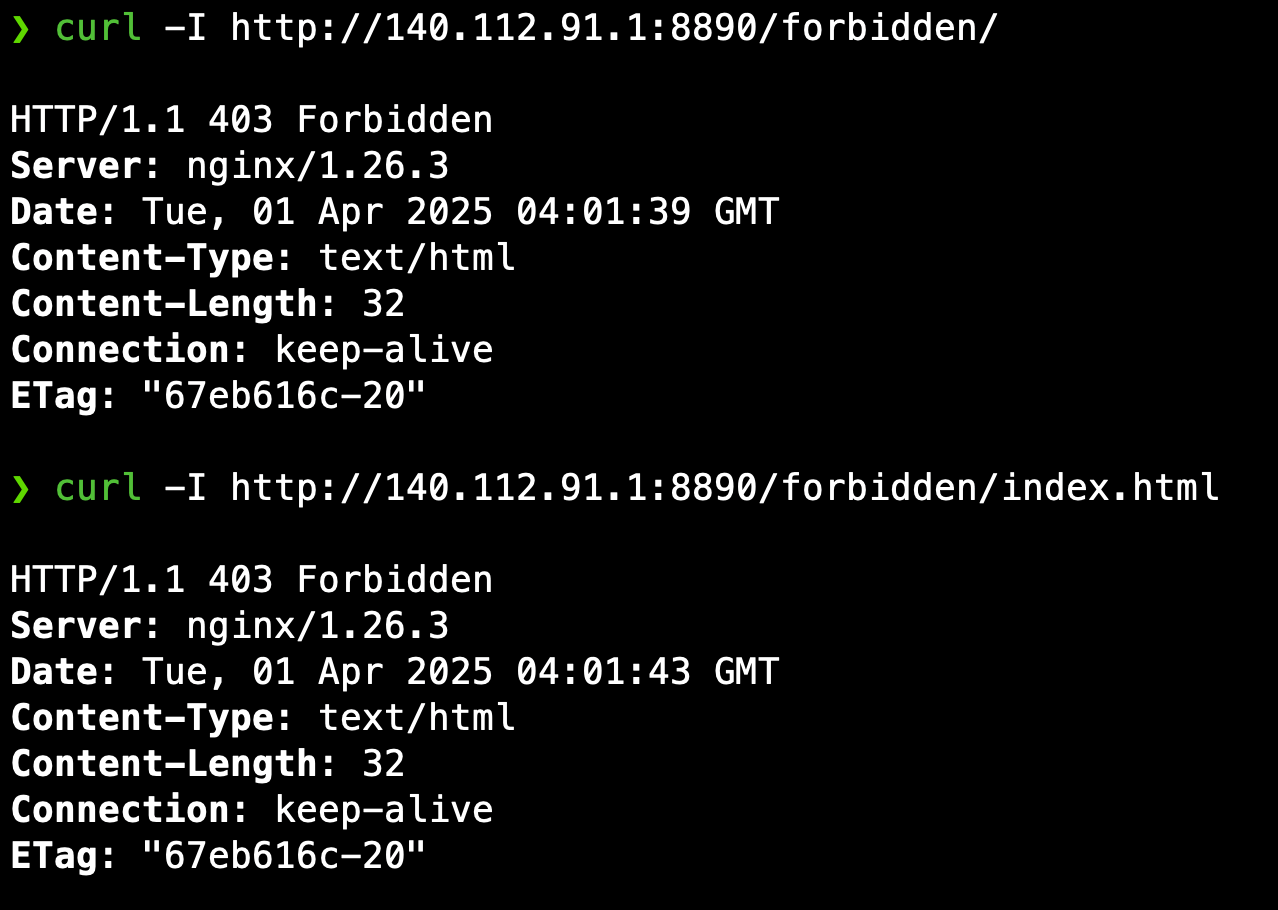
\includegraphics[width=0.5\textwidth]{2-3-1.png}
    \caption{test http status code}
  \end{figure}
  \item 接著，我在瀏覽器上輸入 \texttt{140.112.91.1:8890/forbidden}，可以看到我建立的 403 頁面。
  \begin{figure}[H]
    \centering
    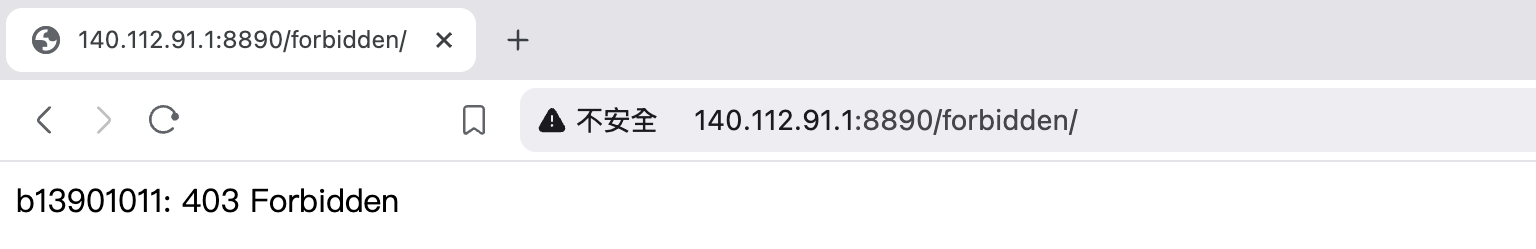
\includegraphics[width=0.7\textwidth]{2-3-2.png}
    \caption{403 Forbidden Page}
  \end{figure}
\end{enumerate}

\subsection{User directory}
\begin{enumerate}
  \item 我可以編輯 \texttt{/etc/skel} 資料夾中的檔案，讓新建立的使用者可以擁有預設的檔案。這些檔案會在新使用者建立時自動複製到新使用者的家目錄中。
  \begin{minted}{bash}
    sudo mkdir /etc/skel/htdocs
    sudo chmod 755 /etc/skel/htdocs
  \end{minted}
  \item 在 \texttt{/etc/nginx/conf.d/default.conf} 中，新增內容如下：
  \begin{minted}{nginx}
    location ~ ^/~(.+?)(/.*)?$ {
      alias /home/$1/htdocs$2;
      index  index.html index.htm index.php;
      autoindex on;
    }
  \end{minted}
  \item 重啟 Nginx 服務。
  \begin{minted}{bash}
    sudo systemctl restart nginx
  \end{minted}
  \item 在 VM 上建立一個新的使用者：
  \begin{minted}{bash}
    sudo adduser user1
    sudo chmod 711 /home/user1
  \end{minted}
  建立完成後，可以發現裡面內建了 \texttt{htdocs} 資料夾，並且可以在裡面建立檔案。
  \begin{figure}[H]
    \centering
    
\includegraphics[width=0.7\textwidth]{2-4-1.png}
    \caption{UserDir}
  \end{figure}
  \item 在 \texttt{htdocs} 資料夾中建立一個 index.html 檔案，內容如下：
  \begin{minted}{bash}
    sudo echo "<p>user1: UserDir</p>" > /home/user1/htdocs/index.html
  \end{minted}
  \item 使用瀏覽器，連上 \texttt{140.112.91.1:8890/~user1/}，可以看到我剛剛建立的網頁。
  \begin{figure}[H]
    \centering
    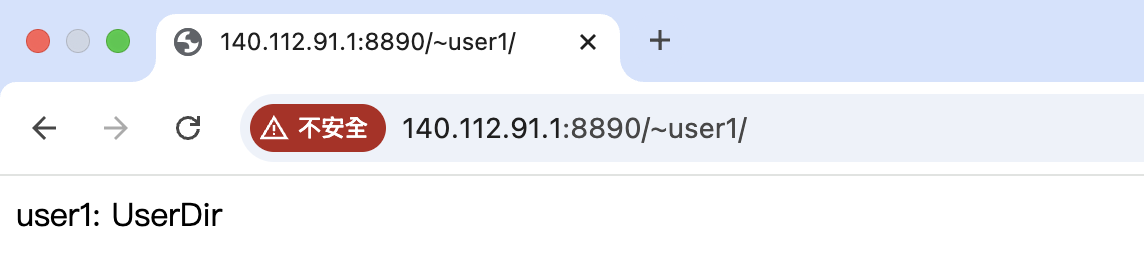
\includegraphics[width=0.8\textwidth]{2-4-2.png}
    \caption{UserDir Page}
  \end{figure}
\end{enumerate}

\subsection{Reverse Proxy}
\begin{enumerate}
  \item 首先，使用以下指令重新開啟 ServerMain VM：
  \begin{minted}{bash}
    qemu-system-x86_64 -enable-kvm -cpu host -m 8G \
      -drive file=debian.qcow2,format=qcow2 \
      -boot d \
      -monitor stdio \
      -nic user,hostfwd=tcp::8890-:80,hostfwd=tcp::1102-:22 \
      -net nic,macaddr=52:54:00:00:00:01 -net vde \
      -vnc :2100,password=on
  \end{minted}
  \item 以 VNC 連線上去，並且打開 terminal，修改 \texttt{/etc/network/interface} 檔案，加入以下內容：
  \begin{minted}{bash}
    auto ens3
    iface ens3 inet static
      address 10.0.2.15/24
      gateway 10.0.2.2
  \end{minted}
  \item 使用以下指令重啟網路服務：
  \begin{minted}{bash}
    sudo systemctl restart networking
  \end{minted}
  \item 建立 ServerA 和 ServerB，我使用先前 Problem 2.1 安裝完的 Debian qcow2 備份檔，複製兩份作為 ServerA 和 ServerB 的 VM，並且使用以下指令開啟 VM：
  \begin{minted}{bash}
    qemu-system-x86_64 -enable-kvm -cpu host -m 8G \
      -drive file=serverA.qcow2,format=qcow2 \
      -boot d \
      -monitor stdio \
      -nic user,hostfwd=tcp::8891-:80,hostfwd=tcp::1103-:22 \
      -net nic,macaddr=52:54:00:00:00:AA -net vde \
      -vnc :2200,password=on
  \end{minted}
  \vspace{-0.5cm}
  \begin{minted}{bash}
    qemu-system-x86_64 -enable-kvm -cpu host -m 8G \
      -drive file=serverB.qcow2,format=qcow2 \
      -boot d \
      -monitor stdio \
      -nic user,hostfwd=tcp::8892-:80,hostfwd=tcp::1104-:22 \
      -net nic,macaddr=52:54:00:00:00:BB -net vde \
      -vnc :2300,password=on
  \end{minted}
  \item 對於 serverA 和 serverB，重複步驟 2.
  \item 在三台機器上分別 ip a，得到其共通內網 ip 分別為：
  \begin{itemize}
    \item ServerMain: \texttt{192.168.125.218}
    \item ServerA: \texttt{192.168.126.131}
    \item ServerB: \texttt{192.168.126.148}
  \end{itemize}
  同時，我在 ServerA 和 ServerB 上使用 \texttt{curl 192.168.125.218}，可以看到 ServerMain 的網頁，代表它們可以互相連線。
  \item 接著我在 ServerA 和 ServerB 參考 problem 2.1 的步驟安裝 Nginx 和 ufw，並且啟用。
  \item 使用以下指令，在 ServerA 和 ServerB 上建立一個 index.html 檔案
  \begin{minted}{bash}
    # Server A
    sudo mkdir -p /var/www/html/
    sudo echo "<p>I am Server A</p>" > /var/www/html/index.html
    # server B
    sudo mkdir -p /var/www/html/
    sudo echo "<p>I am Server B</p>" > /var/www/html/index.html
  \end{minted}
  \item 修改 ServerA 和 ServerB 的 Nginx 設定檔，將預設的網頁路徑改成我剛剛建立的資料夾。Nginx 的設定檔在 \texttt{/etc/nginx/conf.d/default.conf}。我找到 \texttt{location /} 的設定，修改如下：
  \begin{minted}{nginx}
    location / {
      root   /var/www/html;
      index  index.html index.htm;
    }
  \end{minted}
  接著，重啟 Nginx 服務。
  \begin{minted}{bash}
    sudo systemctl restart nginx
  \end{minted}
  \item 我使用瀏覽器直接連線到 Server A 和 ServerB 的網頁，分別是 \texttt{140.112.91.1:8891} 和 \texttt{140.112.91.1:8892}，可以看到我剛剛建立的網頁。
  \begin{figure}[H]
    \centering
    
\includegraphics[width=0.8\textwidth]{2-5-1.png}
    
\includegraphics[width=0.8\textwidth]{2-5-2.png}
    \caption{Test by directly connecting to Server A and Server B}
  \end{figure}
  \item 回到 ServerMain，設定反向代理，修改設定檔案 \texttt{/etc/nginx/conf.d/default.conf}，在最前面新增以下：
  \begin{minted}{nginx}
    upstream serverA {
      server 192.168.126.131:80;
      keepalive 16;
    }
    upstream serverB {
      server 192.168.126.148:80;
      keepalive 16;
    }
  \end{minted}
  \item 接著，我在 \texttt{server} 區塊的設定中，加入以下內容：
  \begin{minted}{nginx}
    location /serverA/ {
      proxy_pass http://serverA/;
      proxy_set_header Host $host;
      proxy_set_header X-Real-IP $remote_addr;
      proxy_set_header X-Forwarded-For $proxy_add_x_forwarded_for;
      proxy_set_header X-Forwarded-Proto $scheme;
    }

    location /serverB/ {
          proxy_pass http://serverB/;
          proxy_set_header Host $host;
          proxy_set_header X-Real-IP $remote_addr;
          proxy_set_header X-Forwarded-For $proxy_add_x_forwarded_for;
          proxy_set_header X-Forwarded-Proto $scheme;
    }
  \end{minted} 
  \item 以 \texttt{sudo systemctl restart nginx} 重啟 Nginx 服務。
  \item 從瀏覽器當中，分別輸入網址 \texttt{http://140.112.91.1:8890/serverA/} 和\\
   \texttt{http://140.112.91.1:8890/serverB/}，可以看到 Server A 和 Server B 的網頁。
  \begin{figure}[H]
    \centering
    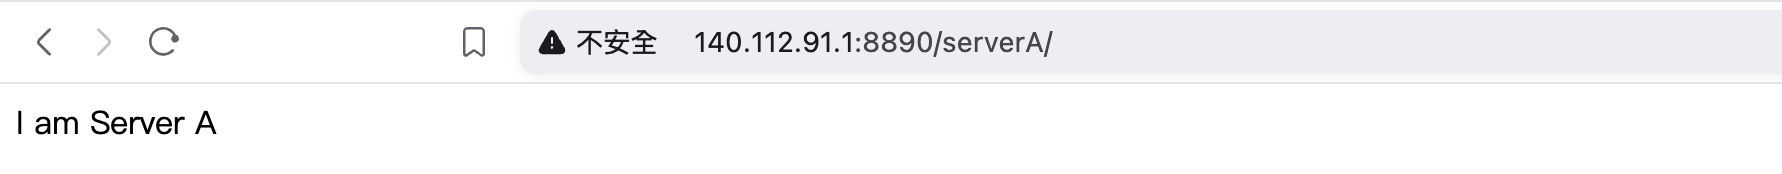
\includegraphics[width=0.8\textwidth]{2-5-3.png}
    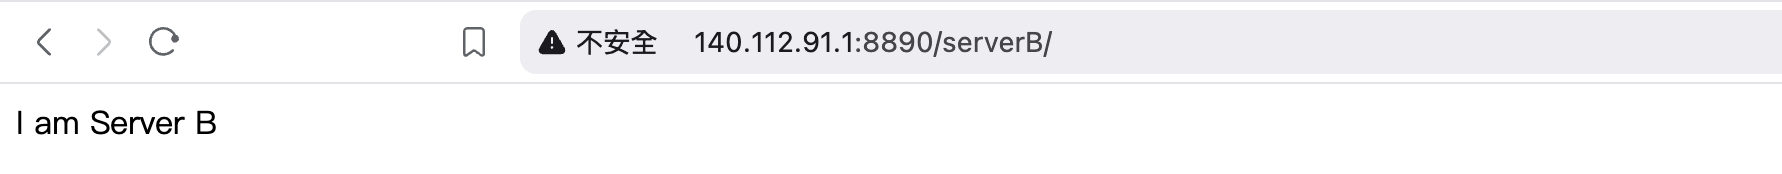
\includegraphics[width=0.8\textwidth]{2-5-4.png}
    \caption{Result of Reverse Proxy}
  \end{figure}
\end{enumerate}

\subsection{Load Balancing}
\begin{itemize}
  \item 將 Server B 的 qcow2 檔案複製一份，並命名為 serverC.qcow2。之後，再以以下指令開啟 VM：
  \begin{minted}{bash}
    qemu-system-x86_64 -enable-kvm -cpu host -m 8G \
      -drive file=serverC.qcow2,format=qcow2 \
      -boot d \
      -monitor stdio \
      -nic user,hostfwd=tcp::8893-:80,hostfwd=tcp::1105-:22 \
      -net nic,macaddr=52:54:00:00:00:CC -net vde \
      -vnc :2400,password=on
  \end{minted}
  \item 此檔案已經設定完網路，並且安裝和啟用過 Nginx 和 ufw，我使用 \texttt{ip a} 來獲 Server C 在 VDE 網路中的 IP 位址為 \texttt{192.168.126.165}。
  \item 接著，我去修改 Server C 的 \texttt{/var/www/html/index.html} 檔案，內容如下：
  \begin{minted}{html}
    <p>I am Server C</p>
  \end{minted}
  之後，並重新啟動 Nginx 服務。
  \begin{minted}{bash}
    sudo systemctl restart nginx
  \end{minted}
  \item 回到 ServerMain，修改 \texttt{/etc/nginx/conf.d/default.conf} 的設定檔，新增一條 upstream 如下：
  \begin{minted}{nginx}
    upstream server {
        server 192.168.126.131:80 max_fails=3 fail_timeout=30s;
        server 192.168.126.148:80 max_fails=3 fail_timeout=30s;
        server 192.168.126.165:80 backup;
    }
  \end{minted}
  \item 接著，我在 \texttt{server} 區塊的設定中，加入以下內容：
  \begin{minted}{nginx}
    location /balance/ {
      proxy_pass http://server/;
      proxy_set_header Host $host;
      proxy_set_header X-Real-IP $remote_addr;
      proxy_set_header X-Forwarded-For $proxy_add_x_forwarded_for;
      proxy_set_header X-Forwarded-Proto $scheme;
    }
  \end{minted}
  \item 以 \texttt{sudo systemctl restart nginx} 重啟 Nginx 服務。
  \item 完成以上之後，我在瀏覽器中以 \texttt{http://140.112.91.1:8890/balance/} 的方式連線到 ServerMain 上的 Nginx 網頁，可以看到 Server A 的網頁，並且重新整理之後可以看到 Server B 的網頁，可以確認成功設定 Round Robin 負載均衡。
  \begin{figure}[H]
    \centering
    
\includegraphics[width=0.9\textwidth]{2-6-1.png}
    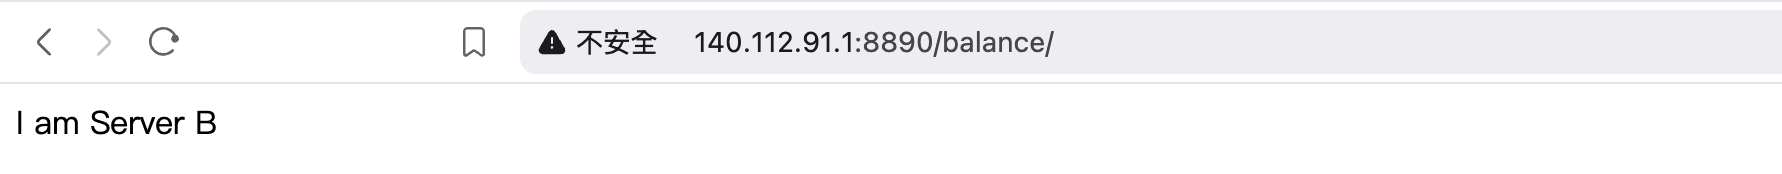
\includegraphics[width=0.9\textwidth]{2-6-2.png}
    \caption{Load Balancing Page}
  \end{figure}
  \item 我關閉 Server A 和 Server B，再重新整理網頁，等待 30 秒左右之後，會發現 Server C 的網頁會顯示出來。
  \begin{figure}[H]
    \centering
    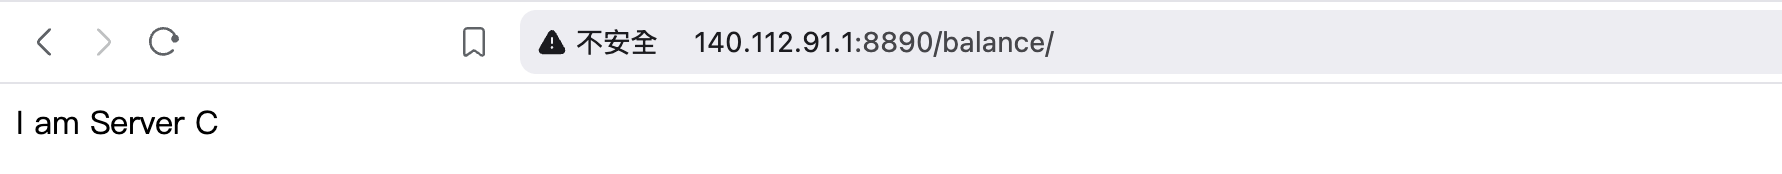
\includegraphics[width=0.9\textwidth]{2-6-3.png}
    \caption{Load Balancing Page}
  \end{figure}
\end{itemize}

\section*{Appendix}
以下附上我在 ServerMain 上的完整 Nginx 設定檔 \texttt{/etc/nginx/conf.d/default.conf} 的內容，包含了每一小題的設定：
\begin{minted}{nginx}
upstream server {
    server 192.168.126.131:80 max_fails=3 fail_timeout=30s;
    server 192.168.126.148:80 max_fails=3 fail_timeout=30s;
    server 192.168.126.165:80 backup;
}

upstream serverA {
    server 192.168.126.131:80;
    keepalive 16;
}

upstream serverB {
    server 192.168.126.148:80;
    keepalive 16;
}
server {
    listen       80;
    server_name  localhost;

    location ~ ^/~(.+?)(/.*)?$ {
            alias /home/$1/htdocs$2;
            index  index.html index.htm;
            autoindex on;
    }

    location / {
            root   /var/www/html;
            index  index.html index.htm;
    }

    location /forbidden/ {
            return 403;
    }

    error_page   403  /403.html;
    location = /403.html {
            root    /var/www/html;
            allow all;
    }

    location /serverA/{
            proxy_pass http://serverA/;
            proxy_set_header Host $host;
            proxy_set_header X-Real-IP $remote_addr;
            proxy_set_header X-Forwarded-For $proxy_add_x_forwarded_for;
            proxy_set_header X-Forwarded-Proto $scheme;
    }
    location /serverB/{
            proxy_pass http://serverB/;
            proxy_set_header Host $host;
            proxy_set_header X-Real-IP $remote_addr;
            proxy_set_header X-Forwarded-For $proxy_add_x_forwarded_for;
            proxy_set_header X-Forwarded-Proto $scheme;
    }

    location /balance/{
            proxy_pass http://server/;
            proxy_set_header Host $host;
            proxy_set_header X-Real-IP $remote_addr;
            proxy_set_header X-Forwarded-For $proxy_add_x_forwarded_for;
            proxy_set_header X-Forwarded-Proto $scheme;
    }

    # redirect server error pages to the static page /50x.html
    #
    error_page   500 502 503 504  /50x.html;
    location = /50x.html {
            root   /usr/share/nginx/html;
    }
}

\end{minted}


% -----------------------------------------------------------
%    You don't have to mess with anything below this line.
% -----------------------------------------------------------

\end{document}
